% Provenance (never printed): cycle 3 / 6e "La planete Terre" (structure of
% the globe: crust, mantle, core); see sources/book1/PROVENANCE.md. Book 1,
% grade 6, chapter 4.
% Vocabulary guard: "magma" not before g7.2 ("molten rock"); P and S waves,
% Moho, core--mantle boundary and lithosphere belong to Book 2 (g11): the
% waves are told in prose, never defined; "seismometer" is defined in g7.3.
\chapter{El interior de la Tierra}\label{ch:g6:inside-the-earth}

En el extremo noroeste de Rusia, no lejos de la frontera con Noruega, hay una tapa de metal soldada al suelo entre edificios abandonados. Debajo, un agujero de solo
unos 23~centímetros de ancho baja en vertical durante más de 12~kilómetros:
es el agujero más profundo jamás excavado. Perforarlo llevó unos 20~años.
Los perforadores esperaban llegar aún más hondo, pero en el fondo la \omterm{def:g3:stones-pebbles-sand:rock}{roca}
estaba a unos 180~grados Celsius, casi el doble de lo previsto: el calor
doblaba las brocas y los tubos, y el trabajo se detuvo en 1992. Y, sin
embargo, el centro de la Tierra está más de \textbf{500 veces} más hondo
que el fondo de ese agujero. ¿Cómo podemos saber lo que hay allí abajo?
% ledger: sciam:kola-depth, sciam:kola-180C, earth:Rmean

\begin{omfigure}
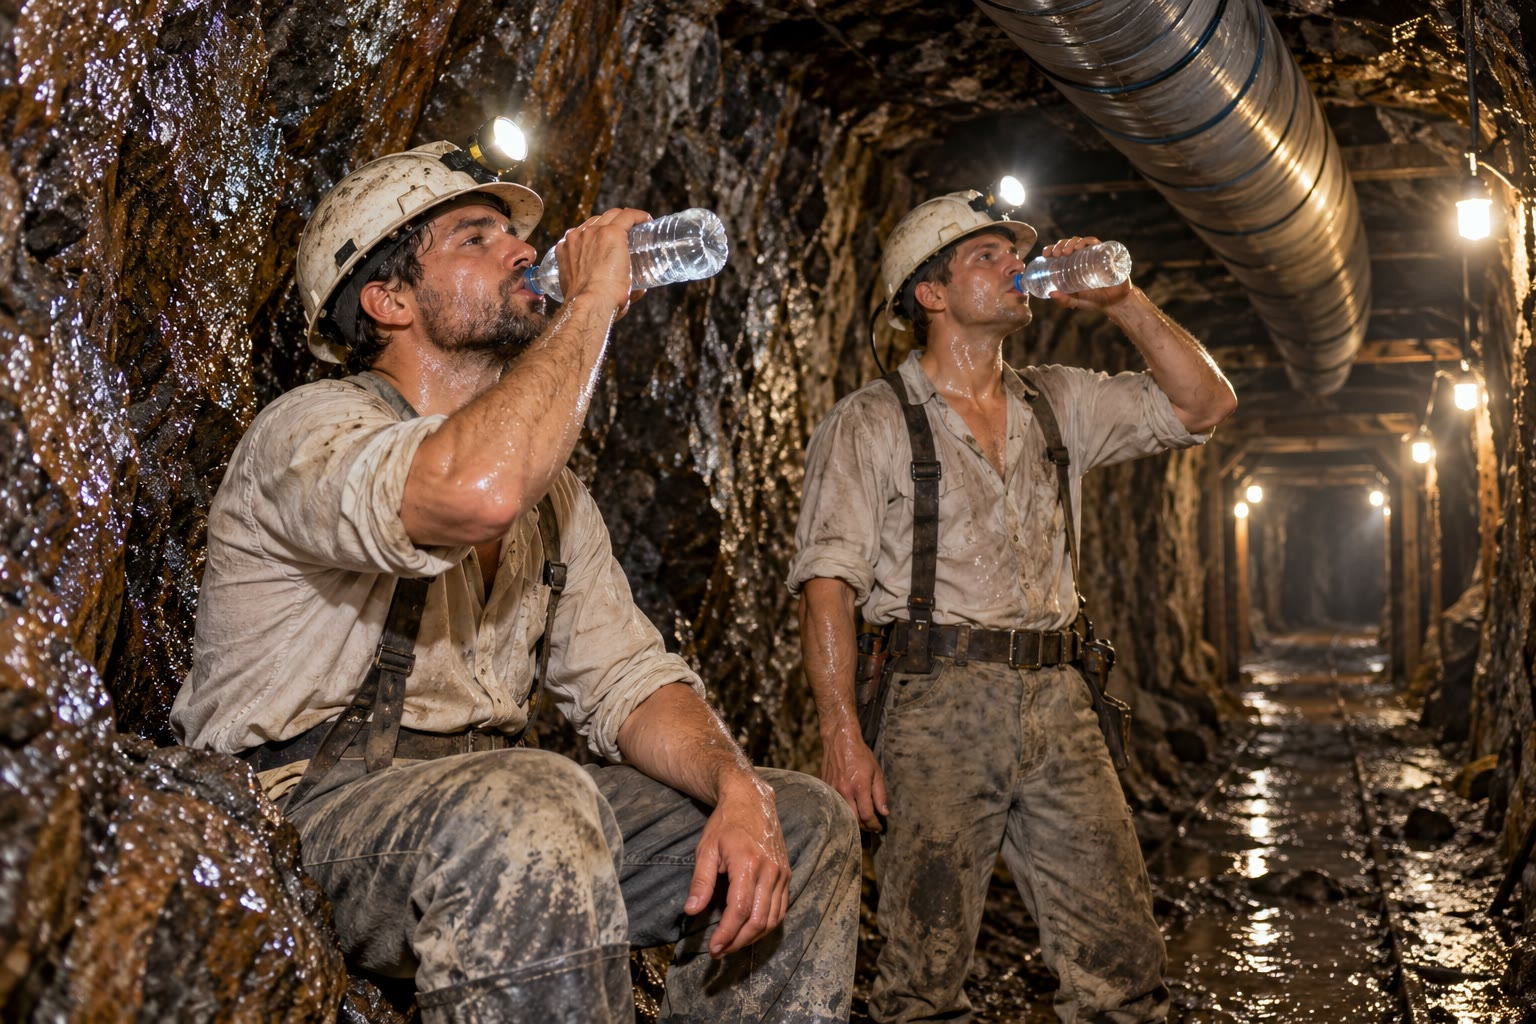
\includegraphics[width=0.62\linewidth]{images/book1/ai/g6-deep-mine.jpg}

{\small Unos mineros beben agua en una galería calurosa, a varios
kilómetros bajo tierra. (Ilustración generada por IA.)}
\end{omfigure}

\begin{recall}
La Tierra es un \omterm{def:g6:earth-a-planet:planet-types}{planeta rocoso}, una bola de unos 12\,742~km de diámetro:
su radio, de la superficie al centro, mide unos 6371~km
(\cref{ch:g6:earth-a-planet}). Sus \omterm{def:g3:stones-pebbles-sand:rock}{rocas} pertenecen a tres familias,
ígneas, sedimentarias y metamórficas (\cref{ch:g6:rocks-and-minerals}). En
un \omterm{def:g4:volcanoes-earthquakes-first-look:volcano}{volcán}, la \omterm{def:g3:stones-pebbles-sand:rock}{roca} fundida sube desde abajo y se derrama en forma de \omterm{def:g4:volcanoes-earthquakes-first-look:eruption}{lava};
en un \omterm{def:g4:volcanoes-earthquakes-first-look:earthquake}{terremoto}, el suelo tiembla (\cref{ch:g4:volcanoes-earthquakes-first-look}).
\end{recall}
% ledger: earth:Rmean

\section{¿Hasta qué profundidad hemos llegado?}

Desde hace mucho tiempo, la gente excava la Tierra en busca de agua, piedra
y metales. Hay dos clases de agujeros que llegan más hondo que los demás.

\textbf{Las minas.} La mina más profunda del mundo es una mina de oro
cercana a Johannesburgo, en Sudáfrica. Sus galerías bajan más de 4~km por
debajo de la superficie. Allí abajo, las paredes de \omterm{def:g3:stones-pebbles-sand:rock}{roca} llegan a unos
60~grados Celsius: la mina se refrigera bombeando hacia abajo miles de
toneladas de hielo mezclado con agua, y con ventiladores gigantes que
soplan aire por las galerías.
% ledger: gwr:deepest-mine

\textbf{Los sondeos.} Un sondeo es un agujero estrecho perforado desde la
superficie con una máquina; nadie baja por él. El más profundo es el sondeo
de la historia del principio, perforado para la ciencia en la península de Kola, en el noroeste de Rusia:
12\,262~metros, es decir, unos 12.3~km.
% ledger: sciam:kola-depth

Estas profundidades parecen enormes. Comparadas con el tamaño de la
Tierra, son diminutas. La figura de abajo las muestra en una sola franja,
junto a la \omterm{def:g1:landscapes-around-us:landform}{montaña} más alta, el Everest (8849~m).
% ledger: tht:everest

\begin{omfigure}
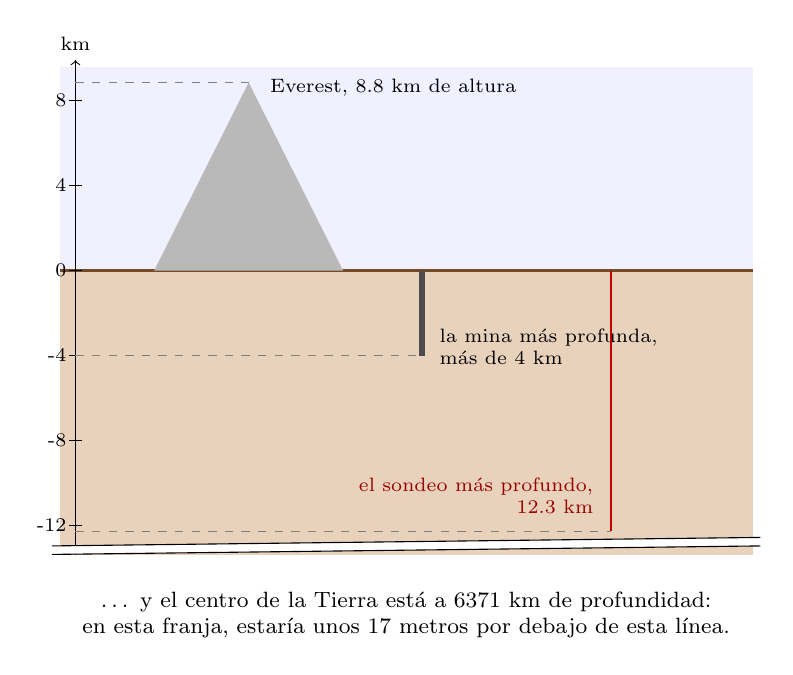
\begin{tikzpicture}[yscale=0.27, xscale=1]
  % sea-level ground and the sky
  \fill[blue!6] (-0.2,0) rectangle (8.6,9.6);
  \fill[brown!35] (-0.2,0) rectangle (8.6,-13.4);
  \draw[thick, brown!60!black] (-0.2,0) -- (8.6,0);
  % depth axis
  \draw[->] (0,-13.4) -- (0,9.9) node[above, font=\scriptsize] {km};
  \foreach \y in {-12,-8,-4,0,4,8} \draw (-0.08,\y) -- (0.08,\y) node[left=2pt, font=\scriptsize] {\y};
  % Everest
  \fill[gray!55] (1.0,0) -- (2.2,8.849) -- (3.4,0) -- cycle;
  \draw[dashed, gray] (0,8.849) -- (2.2,8.849);
  \node[font=\scriptsize, right] at (2.35,8.6) {Everest, 8.8~km de altura};
  % deepest mine
  \draw[line width=2.2pt, black!70] (4.4,0) -- (4.4,-4);
  \draw[dashed, gray] (0,-4) -- (4.4,-4);
  \node[font=\scriptsize, right, align=left] at (4.5,-3.6) {la mina más profunda,\\ más de 4~km};
  % Kola borehole
  \draw[line width=0.7pt, red!75!black] (6.8,0) -- (6.8,-12.262);
  \draw[dashed, gray] (0,-12.262) -- (6.8,-12.262);
  \node[font=\scriptsize, left, align=right, red!60!black] at (6.7,-10.6) {el sondeo más profundo,\\ 12.3~km};
  % break and the centre
  \draw[white, line width=3pt] (-0.3,-13.15) -- (8.7,-12.75);
  \draw (-0.3,-13.35) -- (8.7,-12.95);
  \draw (-0.3,-12.95) -- (8.7,-12.55);
  \node[font=\footnotesize, align=center] at (4.2,-16.2) {\ldots\ y el centro de la Tierra está a 6371~km de profundidad:\\
     en esta franja, estaría unos 17~metros por debajo de esta línea.};
\end{tikzpicture}

{\small Alturas y profundidades dibujadas a la misma escala (1~cm por
3.7~km), desde el \omterm{def:g4:world-physical-map:altitude}{nivel del mar}. El corte de la franja oculta casi todo el
camino hasta el centro.}
% ledger: tht:everest, gwr:deepest-mine, sciam:kola-depth, earth:Rmean
\end{omfigure}

\begin{method}[Comparar una profundidad con el radio de la Tierra]\label{met:g6:inside-the-earth:percent}
\begin{enumerate}
  \item Escribe la profundidad y el radio en la misma unidad (kilómetros).
  \item Divide la profundidad entre el radio y multiplica por 100: así
        obtienes la profundidad como porcentaje del camino hasta el centro.
  \item Para decir cuántas veces más hondo está el centro, divide el radio
        entre la profundidad.
\end{enumerate}
\end{method}

\begin{example}[El sondeo más profundo]\label{ex:g6:inside-the-earth:kola}
El sondeo tiene 12.3~km de profundidad y el radio mide 6371~km.
$12.3 \div 6371 \approx 0.0019$, y $0.0019 \times 100 = 0.19$: el sondeo
recorrió alrededor del \textbf{0.2~\%} del camino hasta el centro. Al
revés, $6371 \div 12.3 \approx 518$: el centro está más de 500~veces más
hondo que el fondo del agujero.

Para la mina más profunda, de unos 4~km: $4 \div 6371 \approx 0.0006$, es
decir, el 0.06~\%: tres veces menos que el sondeo.
% ledger: sciam:kola-depth, earth:Rmean, gwr:deepest-mine
\end{example}

Así que nadie ha visto, tocado ni tomado muestras del interior profundo de
la Tierra. Lo que sabemos de él viene de otras pistas, sobre todo de las
ondas de los \omterm{def:g4:volcanoes-earthquakes-first-look:earthquake}{terremotos} (sección~\ref{sec:g6:inside-the-earth:waves}).

\section{Corteza, manto y núcleo}

La Tierra está construida en capas, un poco como un huevo duro: una
cáscara fina y quebradiza, una ``clara'' gruesa y una ``yema'' en el centro.
% ledger: usgs:layers-egg

\begin{omfigure}
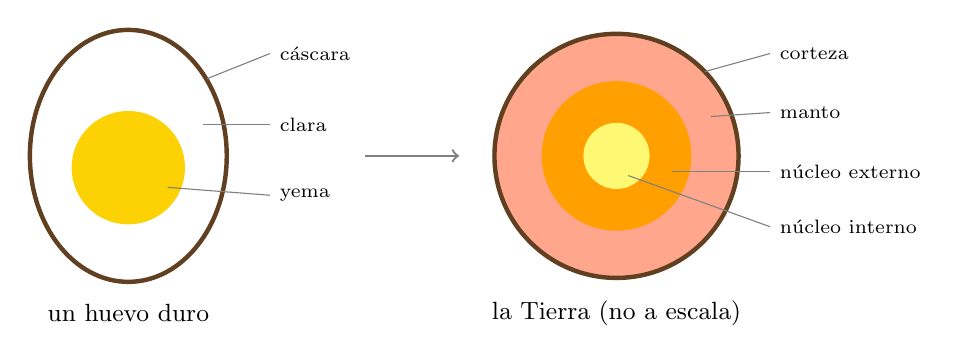
\begin{tikzpicture}
  % a boiled egg cut in half
  \begin{scope}
    \fill[white] (0,0) ellipse (1.25 and 1.6);
    \draw[brown!50!black, line width=1.6pt] (0,0) ellipse (1.25 and 1.6);
    \fill[yellow!70!orange] (0,-0.15) circle (0.72);
    \node[font=\scriptsize, anchor=west] (s) at (1.8,1.3) {cáscara};
    \draw[gray] (s.west) -- (1.0,0.98);
    \node[font=\scriptsize, anchor=west] (w) at (1.8,0.4) {clara};
    \draw[gray] (w.west) -- (0.95,0.4);
    \node[font=\scriptsize, anchor=west] (y) at (1.8,-0.5) {yema};
    \draw[gray] (y.west) -- (0.5,-0.4);
    \node[font=\small] at (0,-2.0) {un huevo duro};
  \end{scope}
  \draw[->, thick, gray] (3.0,0) -- (4.2,0);
  % the Earth, not to scale
  \begin{scope}[xshift=6.2cm]
    \fill[orange!45!red!45] (0,0) circle (1.55);
    \fill[orange!75!yellow] (0,0) circle (0.95);
    \fill[yellow!55] (0,0) circle (0.42);
    \draw[brown!50!black, line width=1.6pt] (0,0) circle (1.55);
    \node[font=\scriptsize, anchor=west] (c) at (1.95,1.3) {corteza};
    \draw[gray] (c.west) -- (1.12,1.07);
    \node[font=\scriptsize, anchor=west] (m) at (1.95,0.55) {manto};
    \draw[gray] (m.west) -- (1.2,0.5);
    \node[font=\scriptsize, anchor=west] (o) at (1.95,-0.2) {núcleo externo};
    \draw[gray] (o.west) -- (0.7,-0.2);
    \node[font=\scriptsize, anchor=west] (i) at (1.95,-0.9) {núcleo interno};
    \draw[gray] (i.west) -- (0.15,-0.25);
    \node[font=\small] at (0,-2.0) {la Tierra (no a escala)};
  \end{scope}
\end{tikzpicture}

{\small La Tierra comparada con un huevo duro. A diferencia de la yema, el
\omterm{def:g6:inside-the-earth:layers}{núcleo} tiene dos partes. En este dibujo la \omterm{def:g6:inside-the-earth:layers}{corteza} aparece mucho más gruesa
de lo que es; el dibujo a escala viene a continuación.}
% ledger: usgs:layers-egg
\end{omfigure}

\begin{definition}[Las capas de la Tierra]\label{def:g6:inside-the-earth:layers}
La Tierra está formada por tres capas principales, de la superficie al
centro:
\begin{itemize}
  \item la \emph{corteza}\index{corteza}, una capa exterior fina de \omterm{def:g3:stones-pebbles-sand:rock}{roca}
        sólida, de unos pocos kilómetros a unas pocas decenas de kilómetros
        de espesor;
  \item el \emph{manto}\index{manto}, una capa gruesa de \omterm{def:g3:stones-pebbles-sand:rock}{roca} sólida,
        caliente y densa, que llega hasta unos 2900~km de profundidad;
  \item el \emph{núcleo}\index{nucleo@núcleo}, hecho de metal, sobre todo
        hierro con algo de níquel, desde unos 2900~km hasta el centro. El
        núcleo tiene dos partes: el \emph{núcleo
        externo}\index{nucleo externo@núcleo externo}, que es líquido, y el
        \emph{núcleo interno}\index{nucleo interno@núcleo interno}, una bola
        sólida en el centro, de unos 1220~km de radio.
\end{itemize}
% ledger: usgs:layers-egg, usgs:crust-thickness, data:prem, earth:Rmean
\end{definition}

El dibujo de abajo muestra las capas \emph{a escala}, con los límites
medidos gracias a las ondas de los \omterm{def:g4:volcanoes-earthquakes-first-look:earthquake}{terremotos}.

\begin{omfigure}
\pgfplotstableread{figdata/out/grade-6-earth_layers-disc.dat}\disctab
\pgfplotstablegetelem{0}{r_cm}\of\disctab \let\rE\pgfplotsretval
\pgfplotstablegetelem{1}{r_cm}\of\disctab \let\rOC\pgfplotsretval
\pgfplotstablegetelem{2}{r_cm}\of\disctab \let\rIC\pgfplotsretval
\begin{minipage}[c]{0.43\linewidth}\centering
\begin{tikzpicture}
  \fill[orange!45!red!45] (0,0) circle (\rE cm);
  \fill[orange!75!yellow] (0,0) circle (\rOC cm);
  \fill[yellow!55] (0,0) circle (\rIC cm);
  \draw[brown!50!black, line width=0.45pt] (0,0) circle (\rE cm);
  
  \draw[gray, thin] (-0.25,\rE) rectangle (0.25,\rE-0.12);
  
  \node[font=\scriptsize, align=center, inner sep=0pt] at (0,0) {núcleo\\ interno};
  \node[font=\scriptsize, align=center] at (0,1.03) {núcleo\\ externo};
  \node[font=\scriptsize] at (0,2.12) {manto};
  \draw[<-, font=\scriptsize] (1.98,1.98) -- (2.3,2.75) node[above, align=center] {corteza\\ (un trazo finísimo)};
\end{tikzpicture}
\end{minipage}\hfill
\begin{minipage}[c]{0.55\linewidth}\centering
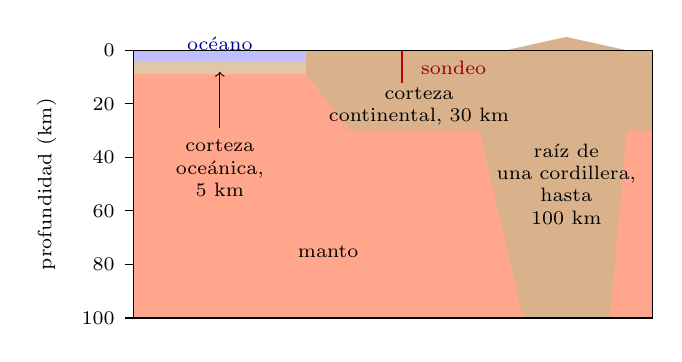
\begin{tikzpicture}[yscale=0.034, xscale=0.55]
  % the top 100 km enlarged: ocean on the left, continent and a range on the right
  \fill[orange!45!red!45] (0,0) rectangle (12,-100);
  \fill[blue!25] (0,0) rectangle (4,-4);
  \fill[brown!45] (0,-4) rectangle (4,-9);                 % oceanic crust 5 km
  \fill[brown!60] (4,0) -- (4,-9) -- (5,-30) -- (8,-30) -- (9,-100) -- (11,-100) -- (11.4,-30) -- (12,-30) -- (12,0) -- cycle;
  \fill[brown!60] (8.6,0) -- (10,5) -- (11.4,0) -- cycle;   % the range (not to scale above ground)
  \draw[red!75!black, line width=0.8pt] (6.2,0) -- (6.2,-12.262);
  \draw[thin] (0,0) rectangle (12,-100);
  \foreach \y in {0,-20,-40,-60,-80,-100} \draw (0,\y) -- (-0.2,\y) node[left, font=\scriptsize] {\pgfmathparse{-\y}\pgfmathprintnumber{\pgfmathresult}};
  \node[font=\scriptsize, rotate=90] at (-2.0,-50) {profundidad (km)};
  \node[font=\scriptsize, align=center] at (2,-44) {corteza\\ oceánica,\\ 5~km};
  \draw[->, thin] (2,-29) -- (2,-8);
  \node[font=\scriptsize, align=center] at (6.6,-21) {corteza\\ continental, 30~km};
  \node[font=\scriptsize, align=center] at (10.0,-50) {raíz de\\ una cordillera,\\ hasta\\ 100~km};
  \node[font=\scriptsize, align=center, red!60!black] at (7.4,-6.5) {sondeo};
  \node[font=\scriptsize] at (4.5,-75) {manto};
  \node[font=\scriptsize, blue!60!black] at (2,2.5) {océano};
\end{tikzpicture}
\end{minipage}

\smallskip
{\small A la izquierda, la Tierra abierta, a escala; el pequeño recuadro
gris de arriba marca la parte ampliada a la derecha. A la derecha, los
100~km de arriba, ampliados unas 60~veces: una \omterm{def:g6:inside-the-earth:layers}{corteza} fina bajo los
\omterm{def:g2:water-on-earth:ocean}{océanos}, más gruesa bajo los \omterm{def:g3:continents-and-oceans:continent}{continentes} y más gruesa aún bajo las altas
\omterm{def:g4:world-physical-map:range}{cordilleras}; en rojo, el sondeo récord.}
% ledger: data:prem, earth:Rmean, usgs:crust-thickness, sciam:kola-depth (figdata/grade-6/earth_layers.py)
\end{omfigure}

\begin{center}\small
\begin{tabular}{|l|c|c|c|l|}
\hline
\textbf{capa} & \textbf{desde (km)} & \textbf{hasta (km)} & \textbf{espesor (km)} & \textbf{hecha de} \\
\hline
\omterm{def:g6:inside-the-earth:layers}{corteza} & 0 & de 5 a 100 & de 5 a 100 & \omterm{def:g3:stones-pebbles-sand:rock}{roca} sólida \\
\omterm{def:g6:inside-the-earth:layers}{manto} & base de la \omterm{def:g6:inside-the-earth:layers}{corteza} & 2891 & unos 2860 & \omterm{def:g3:stones-pebbles-sand:rock}{roca} sólida, muy caliente \\
\omterm{def:g6:inside-the-earth:layers}{núcleo externo} & 2891 & 5150 & unos 2260 & metal líquido \\
\omterm{def:g6:inside-the-earth:layers}{núcleo interno} & 5150 & 6371 (centro) & unos 1220 & metal sólido \\
\hline
\end{tabular}
\end{center}
% ledger: data:prem, usgs:crust-thickness, usgs:layers-egg, earth:Rmean (figdata/grade-6/earth_layers.py, main table)

\textbf{La \omterm{def:g6:inside-the-earth:layers}{corteza}} es la única capa sobre la que podemos caminar y en la
que podemos excavar. Es muy fina comparada con las demás: bajo los \omterm{def:g2:water-on-earth:ocean}{océanos}
solo tiene unos 5~km de espesor; bajo los \omterm{def:g3:continents-and-oceans:continent}{continentes}, unos 30~km de media;
bajo las altas \omterm{def:g4:world-physical-map:range}{cordilleras} como los Alpes, su base puede llegar a 100~km de
profundidad, como la raíz de una muela. Ni siquiera el sondeo récord, de 12.3~km, atravesó la mitad de una \omterm{def:g6:inside-the-earth:layers}{corteza} continental media. En el dibujo a escala, la \omterm{def:g6:inside-the-earth:layers}{corteza}
es más fina que la línea que rodea el disco.
% ledger: usgs:crust-thickness, sciam:kola-depth

\textbf{El \omterm{def:g6:inside-the-earth:layers}{manto}} es la capa más gruesa: va desde la base de la \omterm{def:g6:inside-the-earth:layers}{corteza}
hasta los 2891~km, alrededor del 45~\% del camino hasta el centro. Su \omterm{def:g3:stones-pebbles-sand:rock}{roca}
es sólida, pero muy caliente y más densa que la \omterm{def:g3:stones-pebbles-sand:rock}{roca} de la \omterm{def:g6:inside-the-earth:layers}{corteza}. A lo
largo de millones de años, la \omterm{def:g3:stones-pebbles-sand:rock}{roca} caliente de una parte del \omterm{def:g6:inside-the-earth:layers}{manto} puede
deslizarse muy despacio, como una pasta muy dura.
% ledger: data:prem, usgs:layers-egg, usgs:lithosphere-80km

\textbf{El \omterm{def:g6:inside-the-earth:layers}{núcleo}} empieza a 2891~km y llega hasta el centro. No está hecho
de \omterm{def:g3:stones-pebbles-sand:rock}{roca}, sino de metal: una aleación de hierro y níquel, casi el doble de
densa que el \omterm{def:g6:inside-the-earth:layers}{manto}. Su parte exterior es \emph{líquida}: un \omterm{def:g2:water-on-earth:ocean}{océano} de metal
fundido de más de 2000~km de profundidad. Su parte interior, desde los
5150~km hasta el centro, es una bola \emph{sólida} de metal, de unos 1220~km de radio: alrededor del 70~\% del ancho de la Luna. Al girar la Tierra, el metal líquido del
\omterm{def:g6:inside-the-earth:layers}{núcleo externo} se mueve, y ese movimiento crea el campo magnético de la
Tierra, el que hace girar la aguja de una brújula.
% ledger: data:prem, usgs:layers-egg, earth:Rmean, planet:Moon.diameter

Cuanto más hondo, más denso. El agua tiene una densidad de 1~gramo por
centímetro cúbico: la \omterm{def:g3:stones-pebbles-sand:rock}{roca} de la \omterm{def:g6:inside-the-earth:layers}{corteza} es entre 2.6 y 2.9 veces más
densa, la \omterm{def:g3:stones-pebbles-sand:rock}{roca} del fondo del \omterm{def:g6:inside-the-earth:layers}{manto} más de 5~veces, y el metal del centro
unas 13~veces (mira el gráfico de abajo). Los materiales más pesados están en el centro y los más ligeros, arriba: la Tierra está ordenada, desde la \omterm{def:g6:inside-the-earth:layers}{corteza} ligera hasta el pesado \omterm{def:g6:inside-the-earth:layers}{núcleo} de metal.
% ledger: data:prem


\begin{omfigure}
\begin{tikzpicture}
  \begin{axis}[omrecord, width=0.86\linewidth, height=5.4cm,
      xmin=0, xmax=6371, ymin=0, ymax=14,
      xlabel={profundidad bajo la superficie (km)},
      ylabel={densidad (g por cm$^3$)},
      xtick={0,1000,2000,3000,4000,5000,6000},
      scaled x ticks=false, x tick label style={/pgf/number format/1000 sep={}},
      clip=false]
    \fill[orange!45!red!20] (axis cs:24.4,0) rectangle (axis cs:2891,14);
    \fill[orange!75!yellow!35] (axis cs:2891,0) rectangle (axis cs:5149.5,14);
    \fill[yellow!30] (axis cs:5149.5,0) rectangle (axis cs:6371,14);
    \addplot[very thick, black] table[x=depth_km, y=rho] {figdata/out/grade-6-earth_layers-profile.dat};
    \node[font=\scriptsize] at (axis cs:1450,12.5) {manto};
    \node[font=\scriptsize] at (axis cs:4020,4.5) {núcleo externo};
    \node[font=\scriptsize] at (axis cs:5760,4.5) {núcleo interno};
    \node[font=\scriptsize, align=left, anchor=west] at (axis cs:80,1.4) {corteza: de 2.6 a 2.9};
  \end{axis}
\end{tikzpicture}

{\small Lo densa que es la Tierra a cada profundidad, según un modelo de
referencia construido a partir de mediciones de \omterm{def:g4:volcanoes-earthquakes-first-look:earthquake}{terremotos}. La densidad
salta de unos 5.6 a unos 9.9~g por cm$^3$ donde la \omterm{def:g3:stones-pebbles-sand:rock}{roca} del \omterm{def:g6:inside-the-earth:layers}{manto} deja paso
al metal del \omterm{def:g6:inside-the-earth:layers}{núcleo}.}
% ledger: data:prem (figdata/grade-6/earth_layers.py, part profile)
\end{omfigure}

\begin{inthelab}[Capas en un vaso (en clase, con el profesor)]
El profesor vierte despacio, uno tras otro, en un vaso alto: un poco de
miel, un poco de agua teñida con una gota de tinta y un poco de aceite de
cocina. Sea cual sea el orden en que se vierten, al cabo de un momento la
miel queda en el fondo, el agua en el medio y el aceite arriba: cada
líquido se coloca por debajo de los más ligeros y por encima de los más
densos. Si se agita, el vaso se enturbia; si se deja quieto, vuelve a ordenarse. La Tierra está dividida en capas de la misma manera: el material más denso, el metal del \omterm{def:g6:inside-the-earth:layers}{núcleo}, está en el centro, y la \omterm{def:g3:stones-pebbles-sand:rock}{roca} más ligera, arriba.
\end{inthelab}


\begin{remark}[¿Qué fina es la corteza?]\label{rem:g6:inside-the-earth:thin-crust}
En un \omterm{def:g3:continents-and-oceans:globe}{globo} escolar de 30~cm de diámetro, la \omterm{def:g6:inside-the-earth:layers}{corteza} continental (30~km)
tendría unos 0.7~milímetros de espesor, y la \omterm{def:g6:inside-the-earth:layers}{corteza} oceánica (5~km), más o
menos el grosor de una hoja de papel. La \omterm{def:g6:inside-the-earth:layers}{corteza} es menos de la mitad del
uno por ciento del radio: $30 \div 6371 \approx 0.0047$, es decir, el
0.47~\%.
% ledger: usgs:crust-thickness, earth:Rmean
\end{remark}

\section{Cómo nos cuentan el resto las ondas de los terremotos}\label{sec:g6:inside-the-earth:waves}

Si nadie ha bajado a más de 12~km, ¿cómo podemos dibujar el \omterm{def:g6:inside-the-earth:layers}{núcleo}? La
respuesta viene de los \omterm{def:g4:volcanoes-earthquakes-first-look:earthquake}{terremotos}. Cuando un \omterm{def:g4:volcanoes-earthquakes-first-look:earthquake}{terremoto} sacude el suelo,
salen de él ondas en todas direcciones, que viajan \emph{a través} de toda
la Tierra, igual que el sonido de un golpe viaja a través de una pared. Unos instrumentos situados en muchos lugares del mundo registran cuándo llega cada onda (los conocerás en el
\cref{ch:g7:earthquakes}).
% ledger: data:prem

Las ondas no viajan a la misma velocidad en todos los materiales. Cuando
llegan al límite entre dos capas, su velocidad cambia de golpe: algunas
ondas rebotan y otras se desvían al cruzarlo, un poco como la luz que entra
en el agua. Cronometrando las ondas de muchos \omterm{def:g4:volcanoes-earthquakes-first-look:earthquake}{terremotos}, en estaciones repartidas por todo el \omterm{def:g3:continents-and-oceans:globe}{globo}, los científicos han encontrado dónde están esos límites y
qué capas son sólidas o líquidas. Los sismólogos llaman a las dos clases
principales de ondas \emph{ondas P} (las más rápidas, que empujan y tiran
de la \omterm{def:g3:stones-pebbles-sand:rock}{roca}) y \emph{ondas S} (las más lentas, que la sacuden de un lado a
otro); los volúmenes siguientes las estudian de cerca. Las ondas S tienen
una propiedad notable: no pueden atravesar un líquido.

\begin{omfigure}
\begin{tikzpicture}
  \begin{axis}[omrecord, width=0.86\linewidth, height=5.4cm,
      xmin=0, xmax=6371, ymin=0, ymax=14.5,
      xlabel={profundidad bajo la superficie (km)},
      ylabel={velocidad de las ondas (km por segundo)},
      xtick={0,1000,2000,3000,4000,5000,6000},
      scaled x ticks=false, x tick label style={/pgf/number format/1000 sep={}},
      clip=false]
    \fill[orange!45!red!20] (axis cs:24.4,0) rectangle (axis cs:2891,14.5);
    \fill[orange!75!yellow!35] (axis cs:2891,0) rectangle (axis cs:5149.5,14.5);
    \fill[yellow!30] (axis cs:5149.5,0) rectangle (axis cs:6371,14.5);
    \addplot[very thick, blue!70!black] table[x=depth_km, y=vp] {figdata/out/grade-6-earth_layers-profile.dat};
    \addplot[very thick, red!75!black] table[x=depth_km, y=vs] {figdata/out/grade-6-earth_layers-profile.dat};
    \node[font=\scriptsize, blue!70!black, anchor=south] at (axis cs:1300,12.9) {ondas P (más rápidas)};
    \node[font=\scriptsize, red!75!black, anchor=north] at (axis cs:1500,6.1) {ondas S (más lentas)};
    \node[font=\scriptsize, red!75!black, align=center, fill=white, fill opacity=0.8, text opacity=1] at (axis cs:4020,1.9) {ondas S: 0\\ (líquido)};
    \node[font=\scriptsize] at (axis cs:4020,13.6) {núcleo externo};
    \node[font=\scriptsize] at (axis cs:5760,13.6) {núcleo interno};
    \node[font=\scriptsize] at (axis cs:1450,1.5) {manto};
  \end{axis}
\end{tikzpicture}

{\small La velocidad de las dos clases de ondas de los \omterm{def:g4:volcanoes-earthquakes-first-look:earthquake}{terremotos} a cada
profundidad, en el mismo modelo de referencia. En el \omterm{def:g6:inside-the-earth:layers}{núcleo externo}, las
ondas S se detienen: su velocidad es cero, porque el \omterm{def:g6:inside-the-earth:layers}{núcleo externo} es
líquido.}
% ledger: data:prem (figdata/grade-6/earth_layers.py, part profile)
\end{omfigure}

Leamos el gráfico de izquierda a derecha: en el \omterm{def:g6:inside-the-earth:layers}{manto}, las dos clases de
ondas van cada vez más deprisa con la profundidad. A 2891~km, las ondas S
desaparecen y las ondas P se frenan de golpe: es el techo del \omterm{def:g6:inside-the-earth:layers}{núcleo
externo} líquido. A 5150~km, las ondas P vuelven a acelerar y las ondas S
existen de nuevo: es el \omterm{def:g6:inside-the-earth:layers}{núcleo interno} sólido.
% ledger: data:prem

\begin{history}[Inge Lehmann y el núcleo interno]
\begin{minipage}[c]{0.72\linewidth}
A comienzos de la década de 1930, los sismólogos pensaban que la Tierra tenía dos capas: un \omterm{def:g6:inside-the-earth:layers}{manto} sólido alrededor de un \omterm{def:g6:inside-the-earth:layers}{núcleo} líquido. La sismóloga danesa Inge Lehmann estudió las ondas de un
fuerte \omterm{def:g4:volcanoes-earthquakes-first-look:earthquake}{terremoto} que sacudió Nueva Zelanda en 1929, registradas en
estaciones lejanas. Algunas ondas llegaban a lugares a los que, con un
\omterm{def:g6:inside-the-earth:layers}{núcleo} completamente líquido, no deberían haber llegado nunca. En un
artículo de 1936, titulado sencillamente ``P\,$'$'', propuso una
explicación: dentro del \omterm{def:g6:inside-the-earth:layers}{núcleo} líquido hay un \emph{\omterm{def:g6:inside-the-earth:layers}{núcleo interno} sólido}
más pequeño, que devuelve esas ondas. Escribió con modestia que los datos
eran ``del todo insuficientes'' para estar segura, pero que la
interpretación ``parece posible'', y pidió a otros investigadores que la
pusieran a prueba. Lo hicieron, y hoy el \omterm{def:g6:inside-the-earth:layers}{núcleo interno} sólido forma parte de todos los modelos de referencia de la Tierra, como el que se usa en los gráficos de este capítulo.
% ledger: nbi:lehmann-1936
\end{minipage}\hfill
\begin{minipage}[c]{0.24\linewidth}\centering
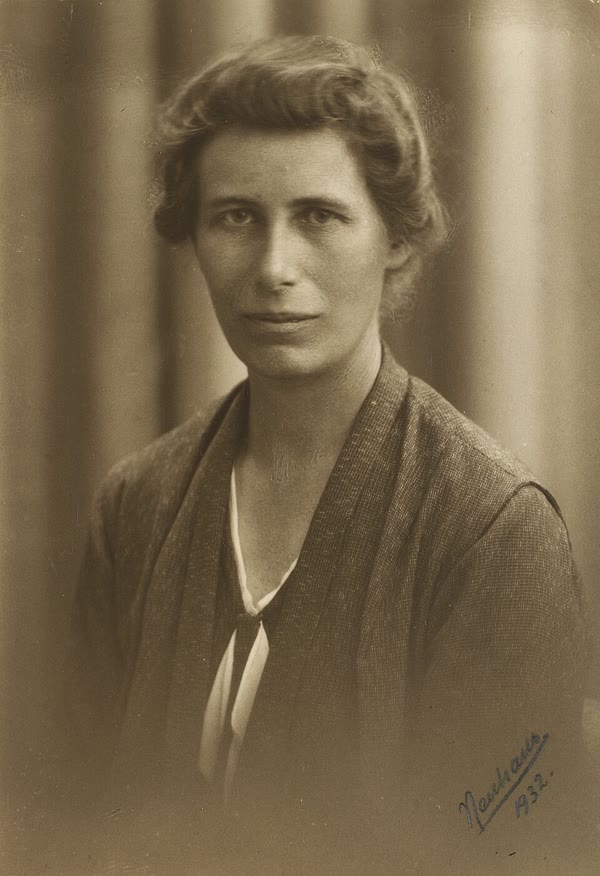
\includegraphics[width=\linewidth]{images/book1/g6-inge-lehmann.jpg}\\[2pt]
{\footnotesize Inge Lehmann en 1932. (Foto: Even Neuhaus, dominio público,
vía Wikimedia Commons.)}
% ledger: commons:inge-lehmann
\end{minipage}
\end{history}

\section{Cuanto más hondo, más calor}

Todas las minas profundas y todos los sondeos profundos muestran lo mismo:
cuanto más se baja, más caliente está la \omterm{def:g3:stones-pebbles-sand:rock}{roca}. En la mina más profunda, las
paredes de \omterm{def:g3:stones-pebbles-sand:rock}{roca} llegan a unos 60~grados Celsius, a más de 4~km de
profundidad; en el fondo del sondeo récord, a 12.3~km, la \omterm{def:g3:stones-pebbles-sand:rock}{roca} estaba a
unos 180~grados.
% ledger: gwr:deepest-mine, sciam:kola-180C

Cerca de la superficie, la temperatura sube a un ritmo bastante regular. En
los Estados Unidos, los científicos reunieron las mediciones de 284
perforaciones, la mayoría de más de 600~m de profundidad. De media, la
temperatura subía \textbf{29~grados por cada kilómetro} de profundidad:
unos 25~grados por kilómetro en el este del país y 34 en el oeste. Pero el
ritmo cambia mucho de un lugar a otro: en esas perforaciones, iba de 6 a
69~grados por kilómetro.
% ledger: usgs:gradient-29

\begin{omfigure}
\begin{tikzpicture}
  \begin{axis}[omrecord, omdepth, width=0.78\linewidth, height=5.6cm,
      xmin=0, xmax=160, ymin=0, ymax=2,
      xlabel={temperatura de la roca ($^\circ$C)},
      ylabel={profundidad (km)},
      ytick={0,0.5,1,1.5,2},
      yticklabel style={/pgf/number format/fixed},
      legend pos=north east, legend cell align=left,
            legend style={font=\scriptsize},
      clip=false]
    \addplot[forget plot, name path=lo, thin, gray] table[x=t_low, y=depth_km] {figdata/out/grade-6-earth_layers-geotherm.dat};
    \addplot[forget plot, name path=hi, thin, gray] table[x=t_high, y=depth_km] {figdata/out/grade-6-earth_layers-geotherm.dat};
    \addplot[forget plot, gray!20] fill between[of=lo and hi];
    \addplot[forget plot, thick, blue!70!black] table[x=t_east, y=depth_km] {figdata/out/grade-6-earth_layers-geotherm.dat};
    \addplot[forget plot, very thick, black] table[x=t_mean, y=depth_km] {figdata/out/grade-6-earth_layers-geotherm.dat};
    \addplot[forget plot, thick, red!75!black] table[x=t_west, y=depth_km] {figdata/out/grade-6-earth_layers-geotherm.dat};
    \addlegendimage{area legend, fill=gray!20, draw=gray}
    \addlegendentry{de 6 a 69 $^\circ$C por km: todas las perforaciones}
    \addlegendimage{thick, blue!70!black}\addlegendentry{25 $^\circ$C por km: este}
    \addlegendimage{very thick, black}\addlegendentry{29 $^\circ$C por km: media}
    \addlegendimage{thick, red!75!black}\addlegendentry{34 $^\circ$C por km: oeste}
  \end{axis}
\end{tikzpicture}

{\small La temperatura según la profundidad (hacia abajo) para un suelo que
empieza a 15~$^\circ$C, con el ritmo medio (29, en negro), las medias del
este y del oeste (25 y 34) y todo el intervalo medido (de 6 a 69, franja
gris). Las mediciones llegan hasta unos 2~km.}
% ledger: usgs:gradient-29, planet:Earth.Tmean (figdata/grade-6/earth_layers.py, part geotherm)
\end{omfigure}

\begin{method}[La temperatura a una profundidad]\label{met:g6:inside-the-earth:temperature}
\begin{enumerate}
  \item Toma la temperatura del suelo cerca de la superficie.
  \item Multiplica la profundidad, en kilómetros, por el ritmo, en grados
        por kilómetro: es lo que se calienta de más.
  \item Suma las dos cosas. Úsalo solo en el intervalo en el que se midió
        el ritmo: unos pocos kilómetros.
\end{enumerate}
\end{method}

\begin{example}[A dos kilómetros de profundidad]\label{ex:g6:inside-the-earth:two-km}
El suelo está a 15~$^\circ$C y el ritmo es de 29~grados por kilómetro. A
2~km: $2 \times 29 = 58$ grados más, así que $15 + 58 = 73~^\circ$C: más
caliente que el baño más caliente, y ya demasiado caliente para tocarlo.
% ledger: usgs:gradient-29, planet:Earth.Tmean
\end{example}

¿Se puede usar el mismo ritmo hasta el centro? No. A 29~grados por
kilómetro, el centro estaría a unos 185\,000~grados, lo cual es
imposible: el ritmo medido en los primeros kilómetros no vale en las profundidades, donde la subida tiene que ser mucho más lenta. Los científicos estiman la temperatura
del \omterm{def:g6:inside-the-earth:layers}{núcleo} de otra manera: en el laboratorio, aprietan granos diminutos
de hierro entre dos diamantes, hasta millones de veces la presión del
aire, y los calientan con láseres hasta que se funden. Así descubrieron
que en el borde del \omterm{def:g6:inside-the-earth:layers}{núcleo interno} sólido la temperatura es de unos
\textbf{6000~grados Celsius}, y, sin embargo, el hierro del \omterm{def:g6:inside-the-earth:layers}{núcleo interno} sigue sólido, porque la presión que hay allí, unos
3.3~millones de veces la presión del aire, le impide fundirse.
% ledger: esrf:core-6000C, usgs:gradient-29

\begin{remark}[Caliente, y aun así sólido]\label{rem:g6:inside-the-earth:pressure}
Si se aprieta mucho una sustancia, solo se funde a una temperatura más
alta. El \omterm{def:g6:inside-the-earth:layers}{manto} está muy caliente, y sin embargo sigue sólido; el \omterm{def:g6:inside-the-earth:layers}{núcleo
externo} es líquido; el \omterm{def:g6:inside-the-earth:layers}{núcleo interno}, aún más caliente, vuelve a ser
sólido, porque es el más apretado de todos. Que algo se funda o no depende
de la temperatura \emph{y} de la presión.
% ledger: esrf:core-6000C, data:prem
\end{remark}

\section{Ejercicios}

\begin{exercise}[$\star$]\label{exo:g6:inside-the-earth:1}
Nombra en orden las cuatro capas de la Tierra, de la superficie al centro.
¿Cuál es líquida? ¿Cuáles están hechas de metal?
\end{exercise}

\begin{exercise}[$\star$]\label{exo:g6:inside-the-earth:2}
¿Verdadero o falso? Corrige las frases falsas.
(a) La \omterm{def:g6:inside-the-earth:layers}{corteza} es más gruesa bajo los \omterm{def:g2:water-on-earth:ocean}{océanos} que bajo los \omterm{def:g3:continents-and-oceans:continent}{continentes}.
(b) El \omterm{def:g6:inside-the-earth:layers}{núcleo} está hecho de \omterm{def:g3:stones-pebbles-sand:rock}{roca}.
(c) El \omterm{def:g6:inside-the-earth:layers}{núcleo interno} es sólido.
(d) El sondeo más profundo jamás perforado tiene unos 12~km de profundidad.
\end{exercise}

\begin{exercise}[$\star$]\label{exo:g6:inside-the-earth:3}
Usa la tabla de las capas. (a) ¿A qué profundidad empieza el \omterm{def:g6:inside-the-earth:layers}{núcleo}?
(b) ¿A qué profundidad empieza el \omterm{def:g6:inside-the-earth:layers}{núcleo interno}? (c) ¿Qué espesor tiene el
\omterm{def:g6:inside-the-earth:layers}{núcleo externo}?
\end{exercise}

\begin{exercise}[$\star$]\label{exo:g6:inside-the-earth:4}
A menudo se compara la Tierra con un huevo duro. Copia y completa: ``La
cáscara es como la \ldots, la clara es como el \ldots{} y la yema es como
el \ldots{}. Pero, a diferencia de la yema, el \ldots{} tiene dos partes:
un \ldots{} líquido y un \ldots{} sólido''.
\end{exercise}

\begin{exercise}[$\star\star$]\label{exo:g6:inside-the-earth:5}
El Everest mide 8.849~km de altura y el radio de la Tierra, 6371~km. ¿Qué
porcentaje del radio representa la altura del Everest? Redondea a dos
decimales. Vista desde lejos, ¿tiene la superficie de la Tierra muchos
bultos?
\end{exercise}

\begin{exercise}[$\star\star$]\label{exo:g6:inside-the-earth:6}
La \omterm{def:g6:inside-the-earth:layers}{corteza} continental tiene 30~km de espesor de media, y la \omterm{def:g6:inside-the-earth:layers}{corteza}
oceánica, 5~km. (a) ¿Cuántas veces más gruesa es la \omterm{def:g6:inside-the-earth:layers}{corteza} continental?
(b) Bajo una alta \omterm{def:g4:world-physical-map:range}{cordillera}, la \omterm{def:g6:inside-the-earth:layers}{corteza} puede llegar a 100~km. ¿Cuántas
veces más gruesa que la \omterm{def:g6:inside-the-earth:layers}{corteza} oceánica es?
\end{exercise}

\begin{exercise}[$\star\star$]\label{exo:g6:inside-the-earth:7}
En una región, el suelo está a 12~$^\circ$C y la temperatura sube
25~grados por kilómetro. ¿Cuál es la temperatura (a) a 1~km, (b) a
1.5~km, (c) a 2~km?
\end{exercise}

\begin{exercise}[$\star\star$]\label{exo:g6:inside-the-earth:8}
En un sondeo, la \omterm{def:g3:stones-pebbles-sand:rock}{roca} está a 14~$^\circ$C cerca de la superficie y a
74~$^\circ$C a 2~km de profundidad. ¿Cuántos grados sube la temperatura por
cada kilómetro? ¿Está este ritmo entre las medias del este y del oeste de
las mediciones del capítulo?
\end{exercise}

\begin{exercise}[$\star\star$]\label{exo:g6:inside-the-earth:9}
Usa el gráfico de las velocidades de las ondas. (a) ¿Cuál es la velocidad
de las ondas P justo encima del \omterm{def:g6:inside-the-earth:layers}{núcleo}, hacia los 2890~km, y justo por
debajo del techo del \omterm{def:g6:inside-the-earth:layers}{núcleo}? (b) ¿Entre qué profundidades es cero la
velocidad de las ondas S? (c) ¿Qué nos dice esto sobre esa capa?
\end{exercise}

\begin{exercise}[$\star\star$]\label{exo:g6:inside-the-earth:10}
El sondeo récord tiene 12.3~km de profundidad. (a) ¿Qué porcentaje de una
\omterm{def:g6:inside-the-earth:layers}{corteza} continental media (30~km) atravesó? (b) ¿Llegó al \omterm{def:g6:inside-the-earth:layers}{manto}?
\end{exercise}

\begin{exercise}[$\star\star\star$]\label{exo:g6:inside-the-earth:11}
Leo dice: ``Cerca de la superficie, la temperatura sube 29~grados por
kilómetro, así que en el centro, a 6371~km de profundidad, tiene que haber
$15 + 29 \times 6371$ grados''. (a) Calcula el número de Leo. (b) Compáralo
con la temperatura que se ha encontrado en el laboratorio para el borde del
\omterm{def:g6:inside-the-earth:layers}{núcleo interno}. (c) ¿Qué falla en el razonamiento de Leo?
\end{exercise}

\begin{exercise}[$\star\star\star$]\label{exo:g6:inside-the-earth:12}
La Tierra entera tiene una densidad media de unos 5.5~gramos por
centímetro cúbico (\cref{ch:g6:earth-a-planet}), pero las \omterm{def:g3:stones-pebbles-sand:rock}{rocas} de la
\omterm{def:g6:inside-the-earth:layers}{corteza} solo tienen una densidad de 2.6 a 2.9. (a) ¿Qué nos dice esto del
material que hay más abajo? (b) Usa el gráfico de las densidades: ¿en qué capas es la densidad mayor que 5.5 en todas partes? (c) ¿Por qué es lógico que el metal pesado esté en el
centro y no en la superficie?
\end{exercise}

\section{Problema: un viaje al centro, a escala}

\begin{problem}[{Problema de fin de semana --- una Tierra de 2~metros de
diámetro: las capas, los agujeros más profundos y el interior caliente,
dibujados a escala}]
\label{pb:g6:inside-the-earth:1}
% ledger: earth:Rmean, data:prem, usgs:crust-thickness, sciam:kola-depth, tht:everest, usgs:gradient-29, gwr:deepest-mine, esrf:core-6000C
Para la feria del colegio, una clase construye una maqueta de la Tierra
cortada por la mitad, lo más grande posible: la cara plana de la media
bola es un disco de 2~metros de diámetro, pintado con las capas. Todo tiene
que estar a escala. Usa: radio de la Tierra, 6371~km; techo del \omterm{def:g6:inside-the-earth:layers}{núcleo
externo}, 2891~km; techo del \omterm{def:g6:inside-the-earth:layers}{núcleo interno}, 5150~km; \omterm{def:g6:inside-the-earth:layers}{corteza} continental,
30~km; \omterm{def:g6:inside-the-earth:layers}{corteza} oceánica, 5~km; Everest, 8.849~km; sondeo récord, 12.3~km.

\medskip
\noindent\textbf{Parte I --- La maqueta.}
\begin{enumerate}
  \item ¿Cuál es el diámetro de la Tierra, en kilómetros? Escribe el
        diámetro de la maqueta en milímetros.
  \item ¿Cuántos kilómetros de la Tierra real representa 1~milímetro de la
        maqueta? (Divide el diámetro real entre el diámetro de la maqueta.)
  \item En la maqueta, ¿qué altura tiene el Everest, en milímetros?
        Redondea a un decimal.
  \item ¿Qué profundidad tiene el sondeo récord en la maqueta? Compárala
        con la distancia de la superficie al centro de la maqueta.
\end{enumerate}

\medskip
\noindent\textbf{Parte II --- Las capas.}
\begin{enumerate}[resume]
  \item ¿A qué distancia por debajo de la superficie de la maqueta tienen
        que pintar los alumnos el techo del \omterm{def:g6:inside-the-earth:layers}{núcleo externo}? Redondea al
        milímetro más cercano.
  \item La misma pregunta para el techo del \omterm{def:g6:inside-the-earth:layers}{núcleo interno}. ¿Cuál es el
        radio del \omterm{def:g6:inside-the-earth:layers}{núcleo interno} en la maqueta?
  \item ¿Qué capa ocupa más sitio a lo largo de un radio de la maqueta: el
        \omterm{def:g6:inside-the-earth:layers}{manto}, el \omterm{def:g6:inside-the-earth:layers}{núcleo externo} o el \omterm{def:g6:inside-the-earth:layers}{núcleo interno}? Da su espesor en la
        maqueta.
  \item ¿Con qué espesor hay que pintar la \omterm{def:g6:inside-the-earth:layers}{corteza} continental? Redondea a
        un decimal. ¿Es fácil hacerlo con un pincel?
\end{enumerate}

\medskip
\noindent\textbf{Parte III --- El interior caliente.}
\begin{enumerate}[resume]
  \item Los alumnos escriben la temperatura a 2~km, con un suelo a
        15~$^\circ$C y 29~grados por kilómetro. ¿Qué escriben? ¿A qué
        distancia por debajo de la superficie de la maqueta están los
        2~km?
  \item La mina más profunda baja más de 4~km. En la maqueta, ¿es la mina
        más profunda o menos profunda que el sondeo récord? ¿Por unos
        cuántos milímetros?
  \item Cerca del borde del \omterm{def:g6:inside-the-earth:layers}{núcleo interno}, la etiqueta dice ``unos
        6000~$^\circ$C, sólido''. Un visitante se sorprende: ¿por qué el
        \omterm{def:g6:inside-the-earth:layers}{núcleo externo} es líquido y el \omterm{def:g6:inside-the-earth:layers}{núcleo interno}, aún más caliente, es
        sólido?
  \item La \omterm{def:g6:inside-the-earth:layers}{corteza} oceánica es la capa más fina. ¿Qué espesor debe tener en
        la maqueta, en milímetros? Redondea a dos decimales y compáralo con
        el grosor de una hoja de papel (unos 0.1~mm).
\end{enumerate}
\end{problem}
